\documentclass[main.tex]{subfile}
\begin{document}
\section{Delopgave 4\\\normalsize{-- Banker's algorithm til håndtering af deadlocks}}
Formålet med opgaven er, ved brug af den såkaldte Banker's Algorithm, at demonstrere brug af pthreads og hvordan disse kan bruges til at håndtere (og undgå) deadlocks.

\subsection{Implementationen, overordnet set}
Vi tager udgangspunkt i den udleverede kode. For at løse de stillede opgaver har vi foretaget ændringer i main metoden (for at allokere hukommelse til tilstands-structen), samt udfyldt de tomme metoder \texttt{int resource\_request(int i, int *request)} og \texttt{void resource\_release(int i, int *request)}.\\

Vi har derudover oprettet hjælpermetoderne \texttt{int safe\_state(State *s)} og \texttt{int islarger(int *this, int *that, int size)}. Brugen af disse vil blive forklaret nedenfor.

\subsection{De specifikke løsninger}

\subsubsection{Hukommelsesallokering}
I starten af \texttt{main} metoden allokerer vi hukommelsen til tilstands-structen. Efter programmet har modtaget input om antal processer og resourcertyper (\textit{m} og \textit{n}) ved vi hvor meget plads der skal afsættes til vektorerne og matricerne. Dette gøres over 3 omgang: først bliver der allokeret plads til selve structen, derefter til rækkerne i structen (både de 1- og 2-dimensionelle), og til sidst itereres der hen over de 2-dimensionelle rækker i en for-løkke, hvori der allokeres hukommelse til disse.\\

Efter hukommelsesallokeringen kan resten af data indlæses: dette tager den udleverede kode sig af.

\subsubsection{Resource request}
Efter data er indlæst i structen checker vi om der overhovedet er tale om et safe state. Dette check foretages af hjælpefunktionen \texttt{int safe\_state(State *s)} (mere om den nedenfor), og såfrem states \textit{er} safe kører programmet videre: der oprettes en tråd hvori vi kører den udleverede metode \texttt{void *process\_thread(void *param)}. Denne funktion generere en tilfældig request via den udleverede funktion \texttt{void generate\_request(int i, int *request)}, og denne request bruges nu til kalde metoden \texttt{int resource\_request(int i, int *request)}.\\

Her checkes først at den givne request en mindre eller lig med available (ud fra den definition givet i Silberschatz s.327). Såfrem den er ikke er for stor (hvis den er printes en fejlmeddelelse og funktionen returnerer 0), modificeres værdierne \textit{available}, \textit{allocation} og \textit{need} jvf. Resource Request algoritmen. Herefter printes den nye værdi af \textit{allocation} og funktionen returnerer 1.\\

Såfrem det ikke lykkedes at tildele den ønskede resource returnerer funktionen som sagt 0, hvilket i \texttt{void *process\_thread(void *param)} funktionen betyder, at processen sover i et tilfældigt tidsrum, for derefter at forsøge igen.

\subsubsection{Safety algorithm}
Safety algoritmen er defineret i sin egen funktion, tager en reference til et state som parameter, og returnerer 1 eller 0 alt efter om det givne state er safe eller unsafe.\\

Funktionen følger algoritmen som defineret i Silberschatz, og opretter sine egne \texttt{finish}- og \texttt{work} arrays, samt allokerer hukommelse til dem. Herefter går den hver af de 4 steps igennem, og returnerer 1 såfrem alle pladser i \texttt{finish} ender som \textit{true}, 0 og en fejlmeddelelse hvis de ikke gør.

\subsubsection{Resource release}
Efter \texttt{void *process\_thread(void *param)} har behandlet resource requestet genereres der et release hva. \texttt{void generate\_release(int i, int *request)}. Dette release bruges i metoden \texttt{void resource\_release(int i, int *request)} til at 'rulle tilbage' over de samme værdier i structen, som \texttt{int resource\_request(int i, int *request)} tidligere har modificeret.\\

Efter dette er gjort, printes den ny \texttt{allocation}-værdi til terminalen. Processen sover på ny, og gentager derefter sig selv ved at generere en ny request osv.

\subsection{Fejl og mangler}
Umiddelbart kører programmet, men vi oplever at 

\subsection{Test}

\begin{figure}[H]
\center
\fbox{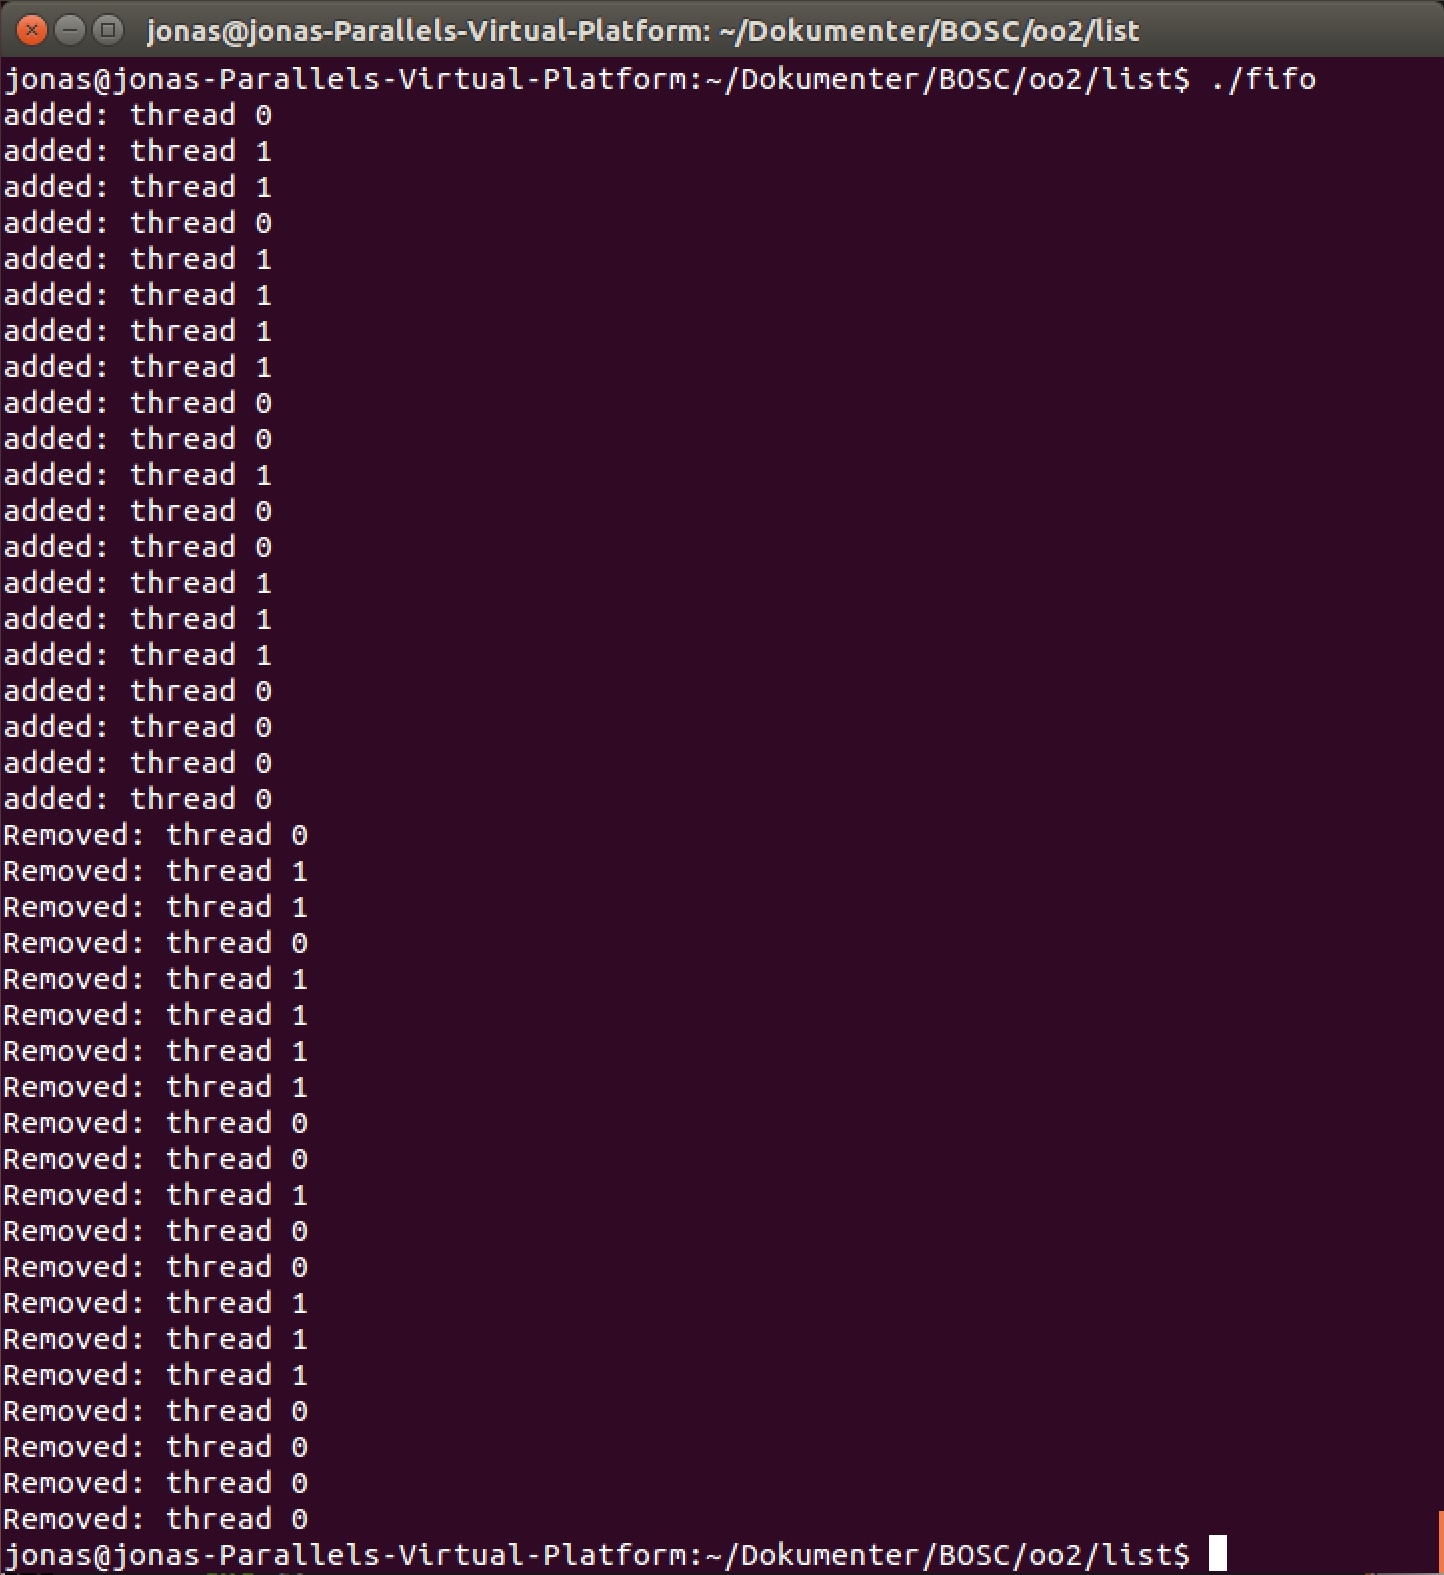
\includegraphics[width=0.85\textwidth]{test_opg_2_2.png}}
\caption{Udskrift af test resultat til terminalen.}

\end{figure}

\end{document}